\pdfminorversion=7
\documentclass[english, usepdftitle=false, svgnames, color="table, fixpdftex, hyperref, fixinclude, xcdraw", t]{beamer}

\usepackage{latexscholar-i18n}
\usepackage{latexscholar-verbatim}
\usepackage{latexscholar-pdf}
\usepackage{lode-imacid}

\usepackage{animate}
\usepackage{movie15}

\title{Software testing}
\subtitle{JUnit}
\author[]{%
	Marco Aur�lio Graciotto Silva\inst{1}, \and
	Ellen Francine Barbosa\inst{2}, \\\and
	Jos� Carlos Maldonado\inst{2}
}

\newcommand{\numberofinstitutes}{2}
\institute[ICMC]
{
	\inst{1}%
	\textbf{Institute of Mathematical Sciences and Computing}\\
	Federal University of Technology -- Paran� (UTFPR)\\
	Campo Mour�o, PR, Brazil
	\and
	\inst{2}%
	\textbf{Institute of Mathematical Sciences and Computing}\\
	University of S�o Paulo (USP)\\
	S�o Carlos, SP, Brazil

}

\date[]{2017}

\logopicture{../CommonAssets/figs/icmc-qualipso-inf.png}

\begin{document}

\frontmatter{}
\begin{frame}[c, plain]
\label{title}
\titlepage
\end{frame}

%\begin{frame}[c,parent={title}, hasprev=false, hasnext=false]
%\frametitle{Software Testing}
%\label{cmap:software-testing}
%
%\insertcmap{Courses-SoftwareTesting-SoftwareTesting}
%\end{frame}

\begin{frame}[c,parent={title}, hasprev=false, hasnext=false]
\frametitle{Software Testing}
\label{cmap:software-testing}

\centering
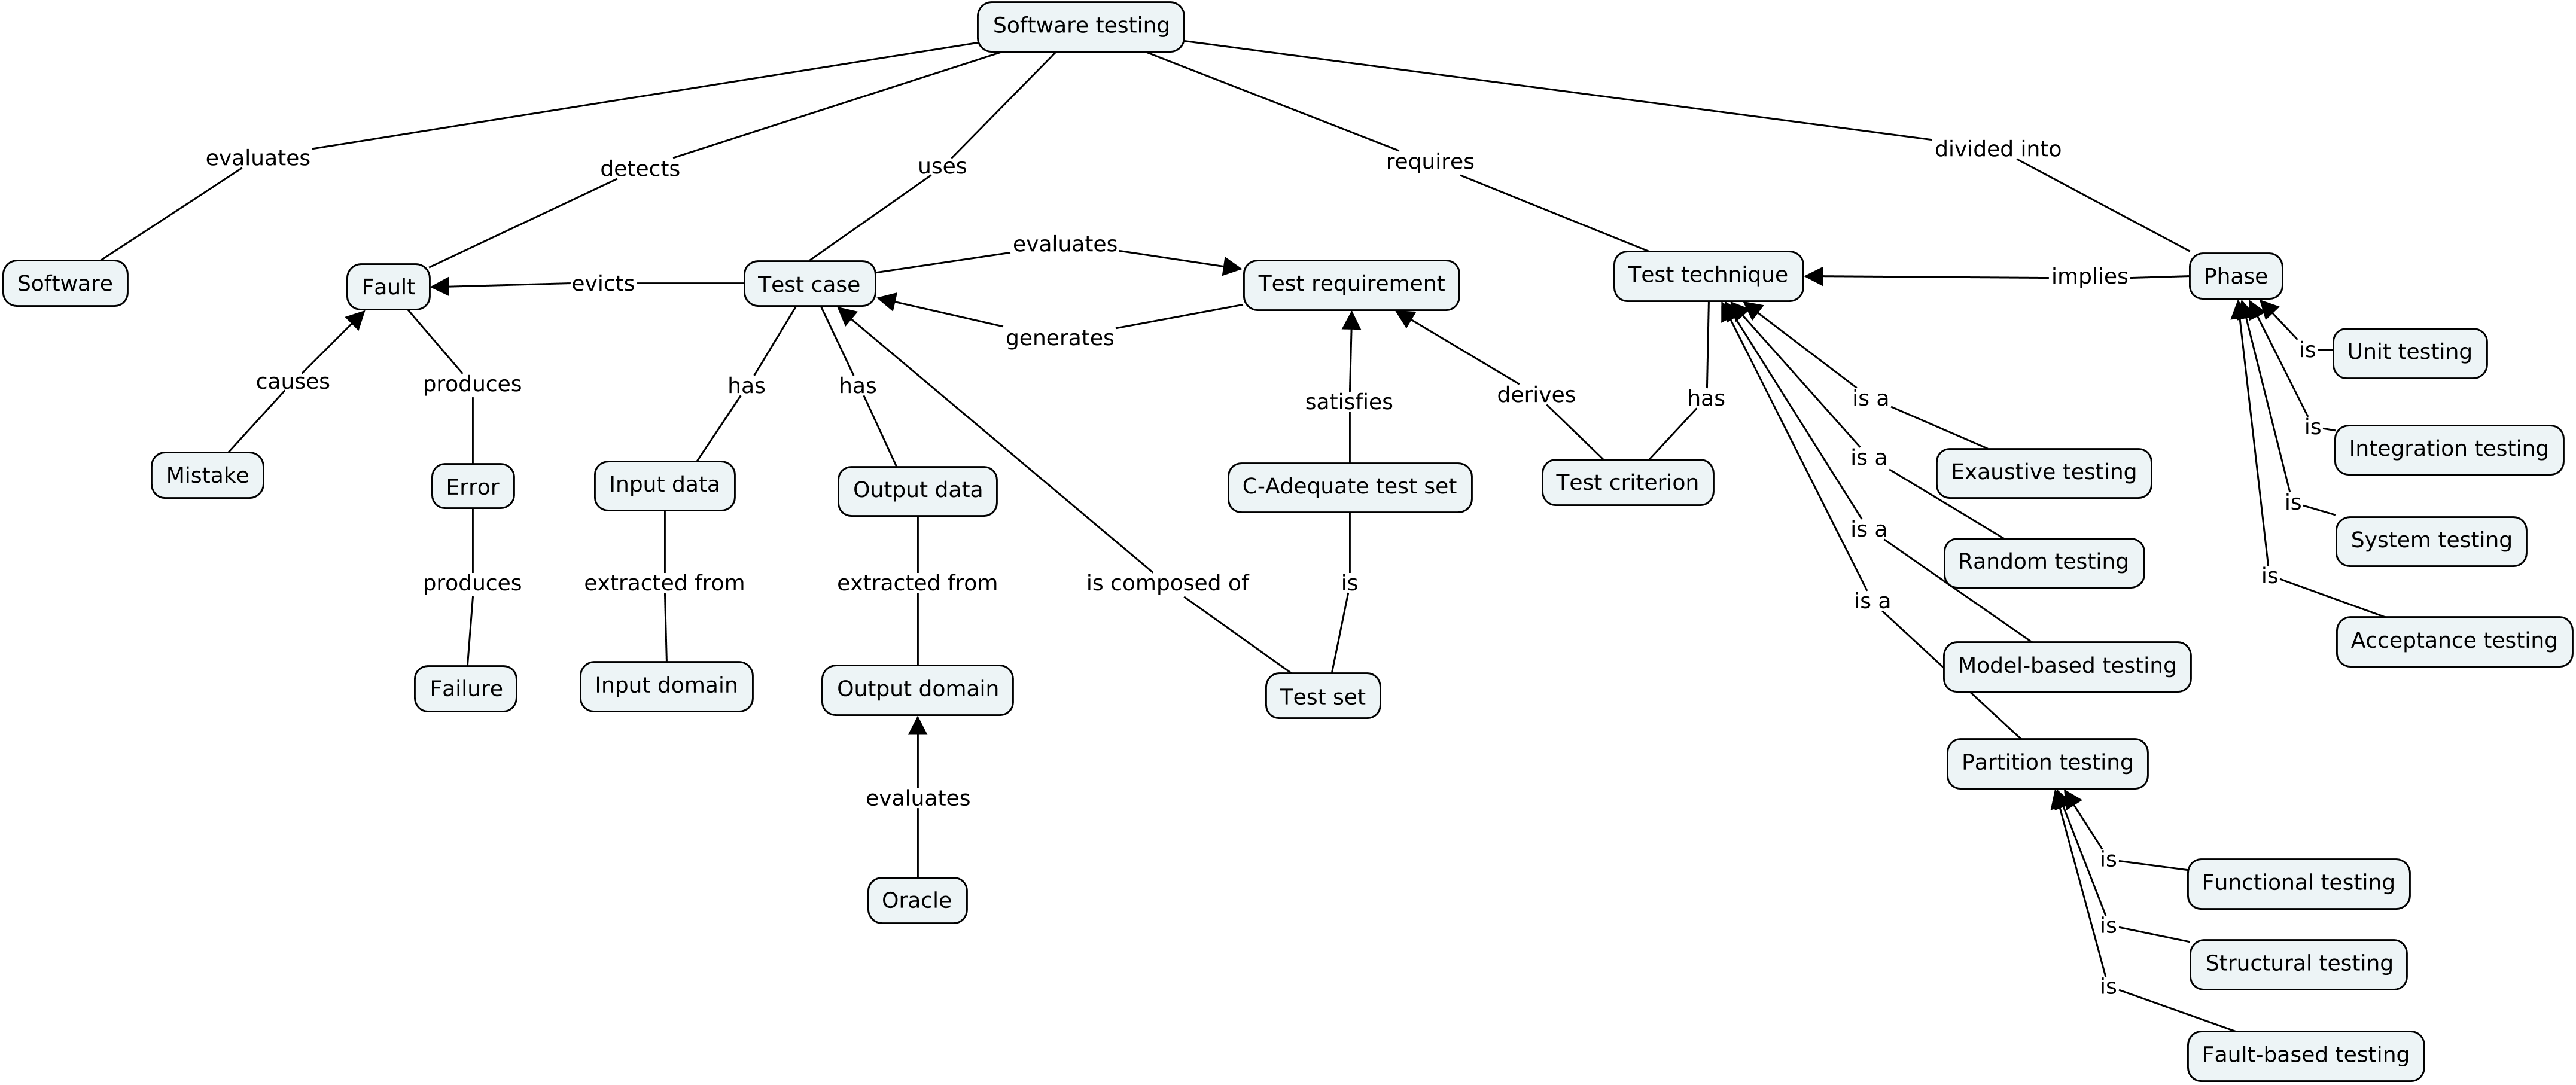
\includegraphics[width=\textwidth]{../BasicConcepts/Software testing fundamentals.png}
\end{frame}




\mainmatter{}
\part{JUnit}
\section{JUnit}
\begin{frame}[c, parent={cmap:software-testing}, hasprev=false, hasnext=true]
\frametitle{JUnit}
\label{cmap:junit}

\insertcmap{Courses-SoftwareTesting-JUnit}
\end{frame}


\begin{frame}[c, parent={cmap:software-testing}, hasprev=true, hasnext=false]
\frametitle{JUnit}
\centering
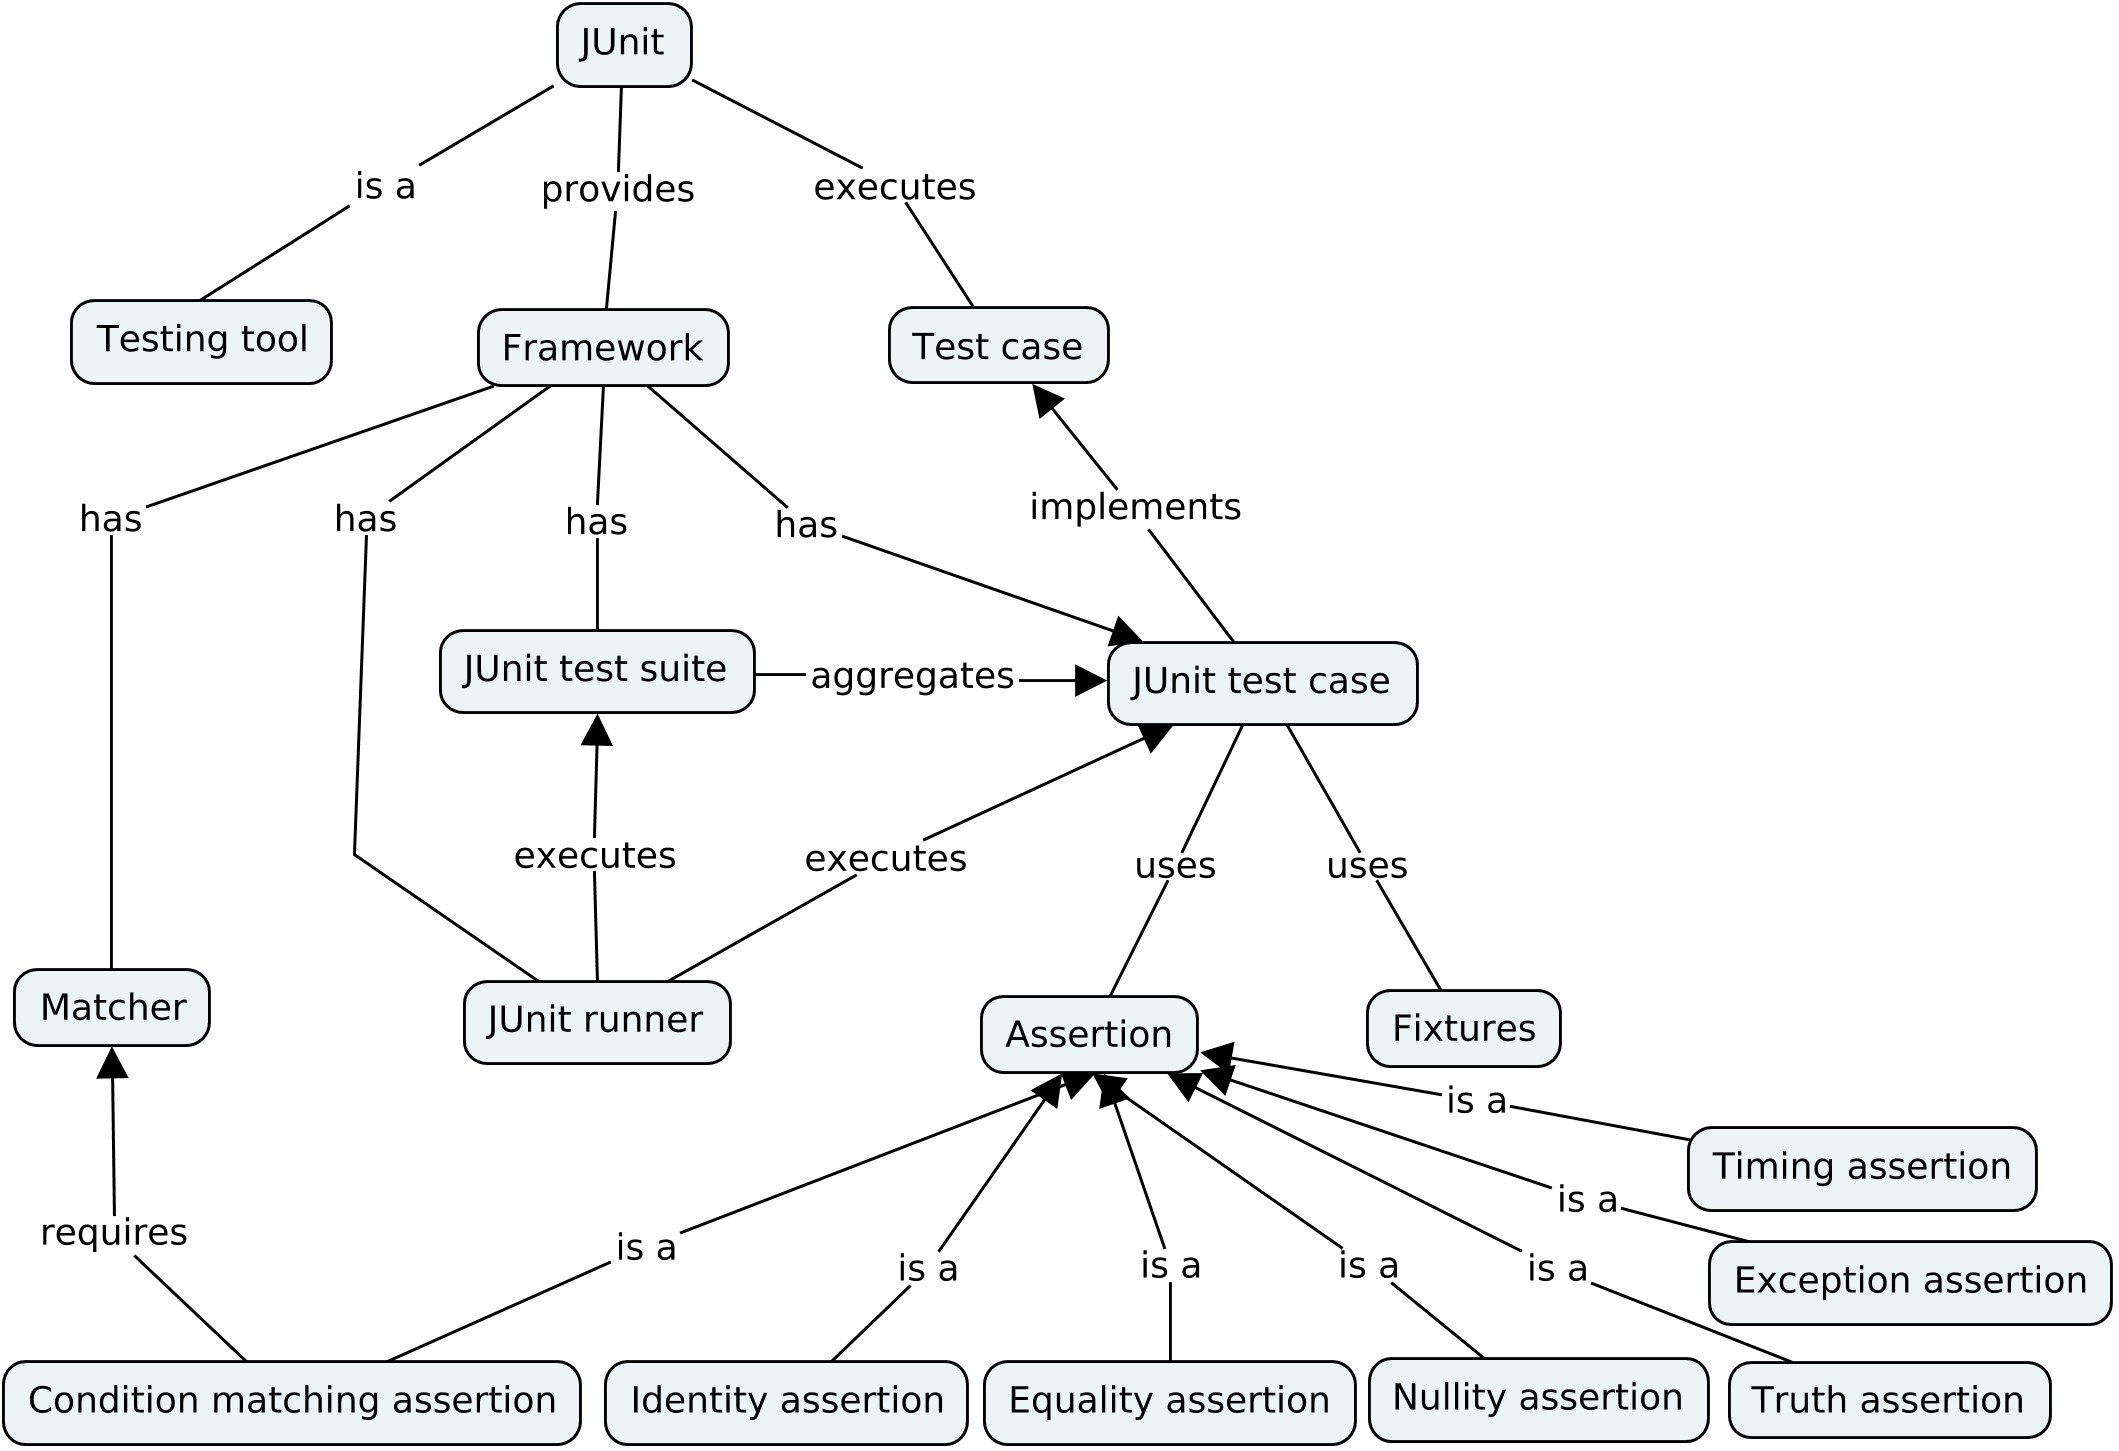
\includegraphics[width=\textwidth]{JUnit.jpg}
\end{frame}


\begin{frame}[parent={cmap:junit}, hasprev=false, hasnext=true]
\frametitle{JUnit}
\label{concept:junit}

\begin{block:concept}{What is it?}
JUnit is an open-source framework to provide support for documenting and
automating the execution of test sets for Java programs.
\end{block:concept}


\begin{block:fact}{General information}
\begin{itemize}
	\item Developed by Kent Beck and Erich Gamma (in 1994).

	\item Hosted at \url{https://www.junit.org/} and
	\url{https://github.com/junit-team/junit4}.
\end{itemize}
\end{block:fact}


\begin{block:fact}{Features}
\begin{itemize}
	\item Test cases implemented using annotations.

	\item Useful assertions collection.

	\item Fixtures enhances the design of test sets.
\end{itemize}
\end{block:fact}

\hfill
\refie{example:identifier-testcases-junit}{\beamerbutton{Example: Identifier}}
\end{frame}





\subsection{Installation}
\begin{frame}[parent={concept:junit}, hasprev=false, hasnext=true]
\frametitle{JUnit}
\framesubtitle{Installation (command line)}
\label{procedure:junit:installation:cmdline}


\begin{block:fact}{Requirements}
\begin{itemize}
	\item JUnit requires the Java SDK 1.5 or newer.
\end{itemize}
\end{block:fact}

\begin{block:procedure}{}
\begin{enumerate}
	\item Download JUnit at \url{https://github.com/junit-team/junit4/wiki/Download-and-Install}.
	\begin{itemize}
		\item Current version is 4.12.

		\item The application is distributed as two JAR files:
		\begin{itemize}
			\item \srccode{junit.jar}: main JUnit library
			\item \srccode{hamcrest-core}: library of matchers (optional, only required for \srccode{assertThat)}
		\end{itemize}
	\end{itemize}
\end{enumerate}
\end{block:procedure}
\end{frame}


\begin{frame}[fragile, hasprev=true, hasnext=true]
\frametitle{JUnit}
\framesubtitle{Installation (command line)}

\begin{block:fact}{Classpath configuration}
	\begin{itemize}
		\item You can add the library to the CLASSPATH environment variable.
\begin{lstlisting}
Unix:
export CLASSPATH=/opt/junit/junit.jar:
  /opt/junit/hamcrest-core.jar:$CLASSPATH
		
Windows:
set CLASSPATH=C:\junit\junit.jar;
  C:\junit\hamcrest-core.jar;%CLASSPATH%
\end{lstlisting}
		
		\item You can use the -cp option when running the tests. This is the
		recommended option!
\begin{lstlisting}
java -cp /opt/junit/junit.jar:/opt/junit/hamcrest-core.jar  <program>
\end{lstlisting}
	\end{itemize}
\end{block:fact}
\end{frame}



\begin{frame}
\frametitle{JUnit}
\framesubtitle{Installation (Eclipse)}
\label{procedure:junit:installation:eclipse}


\begin{block:fact}{Requirements}
	\begin{itemize}
		\item Any Eclipse version
	\end{itemize}
\end{block:fact}

\begin{block:procedure}{}
	For each project you want to use JUnit, proceed as follows:
	\begin{enumerate}
		\item Access the project's properties.
		\item Select \srccode{Java Build Path} tab on the left.
		\item Select \srccode{Libraries} tab on the right.
		\item Select \srccode{Add Library} button on the right of \srccode{Libraries} tab.
		\item Select \srccode{Junit}.
		\item Proceed to the next window by pressing the \srccode{Next button}.
		\item Check if JUnit version is \srccode{JUnit 4}.
		\item Press \srccode{Finish} button.
		\item Press \srccode{Apply} button.
		\item Press \srccode{Ok} button.
	\end{enumerate}
\end{block:procedure}
\end{frame}


\begin{frame}[hasprev=true, hasnext=false]
\frametitle{JUnit}
\framesubtitle{Shake down}
\label{procedure:junit:shakedown}


\begin{block:fact}{Is it working?}
\begin{itemize}
	\item To check whether JUnit was correctly installed, you can run the JUnit
	test suite.
	\begin{itemize}
		\item The class with all the test cases for JUnit is
		\srccode{org.junit.tests.AllTests}.

		\item This class is located at the root of JUnit installation directory.
	\end{itemize}

	\item Or you may create your own test set! Check the example below.
\end{itemize}
\end{block:fact}


\hfill
\refie{example:junit-shakedown}{\beamerbutton{Example: JUnit shakedown}}
\end{frame}



\subsection{Test case}
\begin{frame}[parent={cmap:software-testing-foundations}, hasprev=false, hasnext=true]
\frametitle{Test case}
\label{concept:test-case}
\label{concept:input-domain}
\label{concept:output-domain}
\label{concept:input-data}
\label{concept:output-data}

\begin{block:concept}{Simplified definition}
A test case is a pair consisting of test data (a set of values, one for each
input variable) to be input to the program and the expected output.
\end{block:concept}


\begin{block:concept}{A better definition}
A test case is usually defined as a tuple $(d, S(d))$, where:
\begin{itemize}
	\item $d \in D$ (and $D$ is the input domain), and
	\item $S(d)$ represents the expected output for the input $d$
	according to specification $S$.
\end{itemize}
\end{block:concept}

\hfill
\refie{example:sort-test-cases}{\beamerbutton{Example: Test cases for a sort method}}
\refie{example:num-zero-test-cases}{\beamerbutton{Example: Test cases for the numZero method}}
\end{frame}


\begin{frame}[hasprev=false, hasnext=true]
\frametitle{Test case}
\framesubtitle{Assessing a test case}
\label{concept:test-case-success}
\label{concept:test-case-failure}

\begin{block:fact}{Successful test cases}
\begin{itemize}
	\item At first, a well-constructed and executed test case is successful
	when it finds errors~\cite[p. 7]{myers:2004}

	\item It is also successful when it eventually establishes that there are
	no more errors to be found (as when applying a test criteria and satisfying
	all the test requirements).
\end{itemize}
\end{block:fact}

\begin{block:fact}{Unsuccessful test cases}
\begin{itemize}
	\item A unsuccessful test case is one that causes a program to product the
	correct result without finding any error.
\end{itemize}
\end{block:fact}

\hfill
\refie{example:doctor-laboratory-test}{\beamerbutton{Analogy for test cases success and failure}}
\end{frame}



\begin{frame}
\frametitle{Test case}

\begin{block:fact}{Execution order}
\begin{itemize}
    \item There are two styles of test case design regarding order of test
    execution:
	\begin{itemize}
		\item cascading test cases, and
		\item independent test cases.
	\end{itemize}
\end{itemize}
\end{block:fact}
\end{frame}


\begin{frame}
\label{concept:cascading-test-case}
\frametitle{Test case}
\framesubtitle{Cascading test case}

\begin{block:concept}{Definition}
Cascading test cases are test cases that build on each other.
\end{block:concept}


\begin{block:fact}{Advantages and disadvantages}
\begin{itemize}
	\item The advantage of cascading test cases is that each test case is
	typically small and simple.

	\item The disadvantage of cascading test cases is that if one test fails,
	the subsequent tests may be invalid.
\end{itemize}
\end{block:fact}

\hfill
\refie{example:cascading-test-case}{\beamerbutton{Example: Cascading test cases}}
\end{frame}



\begin{frame}[hasprev=true, hasnext=false]
\label{concept:independent-test-case}
\frametitle{Test case}
\framesubtitle{Independent test case}

\begin{block:concept}{Definition}
Independent test cases are entirely self contained.
\begin{itemize}
	\item Independent test cases neither build on each other nor require that
	other tests have been successfully executed.
\end{itemize}
\end{block:concept}

\begin{block:fact}{Advantages and disadvantages}
\begin{itemize}
	\item The advantage of independent test cases is that any number of tests
	can be executed in any order.

	\item The disadvantage of independent test cases is that each test tends to
	be larger and more complex and thus more difficult to design, create, and
	maintain.
\end{itemize}
\end{block:fact}
\end{frame}


\subsection{Test suite}
\include{main/junit/test-suite}


\subsection{Assertion}
\include{main/junit/assertion}

\subsubsection{Identity assertion}
\include{main/junit/assertion/identity}

\subsubsection{Nullity assertion}
\include{main/junit/assertion/nullity}

\subsubsection{Equality assertion}
\include{main/junit/assertion/equality}

\subsubsection{Exception assertion}
\include{main/junit/assertion/exception}

\subsubsection{Timing assertion}
\include{main/junit/assertion/timing}

\subsubsection{Truth assertion}
\include{main/junit/assertion/truth}

\subsubsection{Condition matching assertion}
\include{main/junit/assertion/condition}


\subsection{Fixture}
\include{main/junit/fixture}

\subsubsection{Before}
\include{main/junit/fixture/before}

\subsubsection{BeforeClass}
\include{main/junit/fixture/before-class}

\subsubsection{After}
\include{main/junit/fixture/after}

\subsubsection{AfterClass}
\include{main/junit/fixture/after-class}



\backmatter{}
\part{References and credits}
\include{bibliography}
\part{Acknowledgement}
\section*{Acknowledgement}


\begin{frame}[c,label=credits]
\frametitle{Credits}

\centering
\animategraphics[height=140pt,poster=first,autoplay,loop]{1}{main/jabuti-}{0}{3}

\begin{itemize}
	\item Reviewers:
	\begin{itemize}
		% \item Auri Marcelo Rizzo Vincenzi
		% \item Ellen Francine Barbosa
		\item Fabiano Cutigi Ferrari
		% \item Márcio Eduardo Delamaro
		\item Otávio Augusto Lazzarini Lemos
	\end{itemize}
\end{itemize}
\end{frame}


\part{Instructional elements}
\include{examples}
\include{exercises}


\end{document}
